

\documentclass[10pt,twocolumn,letterpaper]{article}

%%%%%%%%% PAPER TYPE  - PLEASE UPDATE FOR FINAL VERSION
% \usepackage[review]{cvpr}      % To produce the REVIEW version
\usepackage{cvpr}              % To produce the CAMERA-READY version
%\usepackage[pagenumbers]{cvpr} % To force page numbers, e.g. for an arXiv version

% Include other packages here, before hyperref.
\usepackage{graphicx}
\usepackage{amsmath}
\usepackage{amssymb}
\usepackage{booktabs}
\usepackage[shortlabels]{enumitem}


% It is strongly recommended to use hyperref, especially for the review version.
% hyperref with option pagebackref eases the reviewers' job.
% Please disable hyperref *only* if you encounter grave issues, e.g. with the
% file validation for the camera-ready version.
%
% If you comment hyperref and then uncomment it, you should delete
% ReviewTempalte.aux before re-running LaTeX.
% (Or just hit 'q' on the first LaTeX run, let it finish, and you
%  should be clear).
\usepackage[pagebackref,breaklinks,colorlinks]{hyperref}


% Support for easy cross-referencing
\usepackage[capitalize]{cleveref}
\crefname{section}{Sec.}{Secs.}
\Crefname{section}{Section}{Sections}
\Crefname{table}{Table}{Tables}
\crefname{table}{Tab.}{Tabs.}


%%%%%%%%% PAPER ID  - PLEASE UPDATE
\def\cvprPaperID{*****} % *** Enter the CVPR Paper ID here
\def\confName{CVPR}
\def\confYear{2023}


\begin{document}

%%%%%%%%% TITLE - PLEASE UPDATE
\title{NTIRE 2023 Efficient SR Challenge Factsheet\\PRFDN: High Parallelism Distillation Network For Image Super-resolution}

\author{Daheng Yin, Baijun Chen, Mengyang Liu\\
School of Computer Science and Engineering, Southeast University\\
Nanjing, Jiangsu\\
{\tt\small {yindaheng98, bjchen, myliu}@seu.edu.cn}
% For a paper whose authors are all at the same institution,
% omit the following lines up until the closing ``}''.
% Additional authors and addresses can be added with ``\and'',
% just like the second author.
% To save space, use either the email address or home page, not both
}
\maketitle

\section{Introduction}

This factsheet template is meant to structure the description of the contributions made by each participating team in the NTIRE 2023 challenge on efficient image super-resolution. 

Ideally, all the aspects enumerated below should be addressed.
The provided information, the codes/executables and the achieved performance on the testing data are used to decide the awardees of the NTIRE 2023 challenge. 

Reproducibility is a must and needs to be checked for the final test results in order to qualify for the NTIRE awards. 

The main winners will be decided based on overall performance and a number of awards will go to novel, interesting solutions and to solutions that stand up as the best in a particular subcategory the judging committee will decided. Please check the competition webpage and forums for more details.

The winners, the awardees and the top ranking teams will be invited to co-author the NTIRE 2023 challenge report and to submit papers with their solutions to the NTIRE 2023 workshop. Detailed descriptions are much appreciated.

The factsheet, \href{https://github.com/ofsoundof/NTIRE2023_ESR}{source codes/executables}, trained models should be sent to \textbf{all of the NTIRE 2023 challenge organizers (Yawei Li, Yulun Zhang, and Radu Timofte)} by email.


\section{Email final submission guide}

\noindent To: {yawei.li@vision.ee.ethz.ch} \\ {yulun100@gmail.com} \\ {timofte.radu@gmail.com}\\
\noindent cc: your\_team\_members\\
Title: NTIRE 2023 Efficient SR Challenge - TEAM\_NAME - TEAM\_ID\\

To get your TEAM\_ID, please register at \href{https://docs.google.com/spreadsheets/d/1oekPThh5mq9qKax0hPZiQSHlqTjaoQa-IBfrQkwN7gk/edit?usp=sharing}{Google Sheet}. Please fill in your Team Name, Contact Person, and Contact Email in the first empty row from the top of sheet.
% 
Body contents should include: 

\begin{enumerate}[a)]
\item team name 

\item team leader's name and email address 

\item rest of the team members 

\item user names on NTIRE 2023 CodaLab competitions 

\item Code, pretrained model, and factsheet download command, e.g. \texttt{git clone ...}, \texttt{wget ...}

\item Result download command, e.g. \texttt{wget ...}
\begin{itemize}
    \item Please provide different urls in e) and f)
\end{itemize}
\end{enumerate}



\noindent Factsheet must be a compiled pdf file together with a zip with .tex factsheet source files. Please provide a detailed explanation.


\section{Code Submission}

The code and trained models should be organized according to the \href{https://github.com/ofsoundof/NTIRE2023_ESR}{GitHub repository}. This code repository provides the basis to compare the various methods in the challenge. \textbf{Code scripts based on other repositories will not be accepted.} Specifically, you should follow the steps below.
\begin{enumerate}
    \item Git clone \href{https://github.com/ofsoundof/NTIRE2023_ESR}{the repository.}
    \item Put your model script under the \texttt{models} folder. Name your model script as \texttt{[Your\_Team\_ID]\_[Your\_Model\_Name].py}.
    \item Put your pretrained model under the \texttt{model\_zoo} folder. Name your model checkpoint as \texttt{[Your\_Team\_ID]\_[Your\_Model\_Name].[pth or pt or ckpt]}
    \item Modify \texttt{model\_path} in \texttt{test\_demo.py}. Modify the imported models.
    \item \texttt{python test\_demo.py}
\end{enumerate}
Please send us the command to download your code, e.g. \texttt{git clone [Your repository link]}
When submitting the code, please remove the LR and SR images in \texttt{data} folder to save the bandwidth.

\section{Factsheet Information}

The factsheet should contain the following information. Most importantly, you should describe your method in detail. The training strategy (optimization method, learning rate schedule, and other parameters such as batch size, and patch size) and training data (information about the additional trainning data) should also be explained in detail.

\subsection{Team details}

\begin{itemize}
\item Team name: SEU\_CNII
\item Team leader name: Daheng Yin
\item Team leader address, phone number, and email: \\School of Computer Science and Engineering, Southeast University; \\+86 188 5189 9135; yindaheng98@seu.edu.cn
\item Rest of the team members: Baijun Chen, Mengyang Liu
\item Team website URL (if any): N/A
\item Affiliation: School of Computer Science and Engineering, Southeast University
\item User names and entries on the NTIRE 2023 Codalab competitions (development/validation and testing phases): yindaheng98
\item Best scoring entries of the team during development/validation phase:\\PSNR 28.993
\item Link to the codes/executables of the solution(s): \url{https://github.com/yindaheng98/NTIRE23-RTSR}
\end{itemize}

\subsection{Method details}

We proposed Parallel RFDN (PRFDN) as is shown in figure \ref{fig:PRFDN}.
Our method consists of four stages to transform a pre-trained RFDN\cite{liu2020residual} into PRFDN.
\begin{enumerate}
    \item Branching. To accelerate the inference, we first consider reducing the data dependency in the model to achieve higher parallelism. Our method disentangles the sequentially computed trunks into branches. As is shown in figure \ref{fig:Branching}, after the branching, the major part of the model will consist of four independent branches that can calculate in parallel. To improve the accuracy, we also design a small SR block (SRFDB) based on the RFDB of RFDN and add them before the input of each branch. 
    \item Training. Since we only change the data flow but not the structure of RFDB, the pre-trained RFDN parameters can still be loaded into the major part of our branch model (only except for those SRFDBs). To benefit from the pre-training, we load the pre-trained RFDN parameters into our branch model before training our branch model.
    \item Re-parametrization. Without much data dependency, branches in our model can be computed in parallel. However, a single GPU cannot compute two or more different models in parallel. To address this issue and achieve parallel computing of multiple branches on a single GPU, we should merge the four branches into a single branch. As is shown in figure \ref{fig:Re-parametrization}, we realize that the major part of these four branches (RFDBs and SRFDBs) have exactly the same structure but different parameters, so we merge and re-parametrized the RFDBs and SRFDBs into a single branch. More specifically, we create a bigger RFDB and a bigger SRFDB with bigger convolution layers and move the weight and bias from the RFDBs and SRFDBs into them. After re-parametrization, we get a bigger model that is equivalent to that of the branches of the branch model computed in parallel on a single GPU.
    \item Pruning. The re-parametrized model is big. To further accelerate the inference, we applied channel pruning on our re-parametrized model, as is shown in figure \ref{fig:Pruning}. To accurately extract the channel dependency for pruning, we first replace each concatenate and split operation with an equivalent convolution operation. After replacement, we used Torch-Pruning\cite{fang2023depgraph} to prune the model and finetune the model between each pruning step.
\end{enumerate}

\begin{figure*}
    \centering
    \begin{subfigure}[b]{0.246\linewidth}
		\centering
        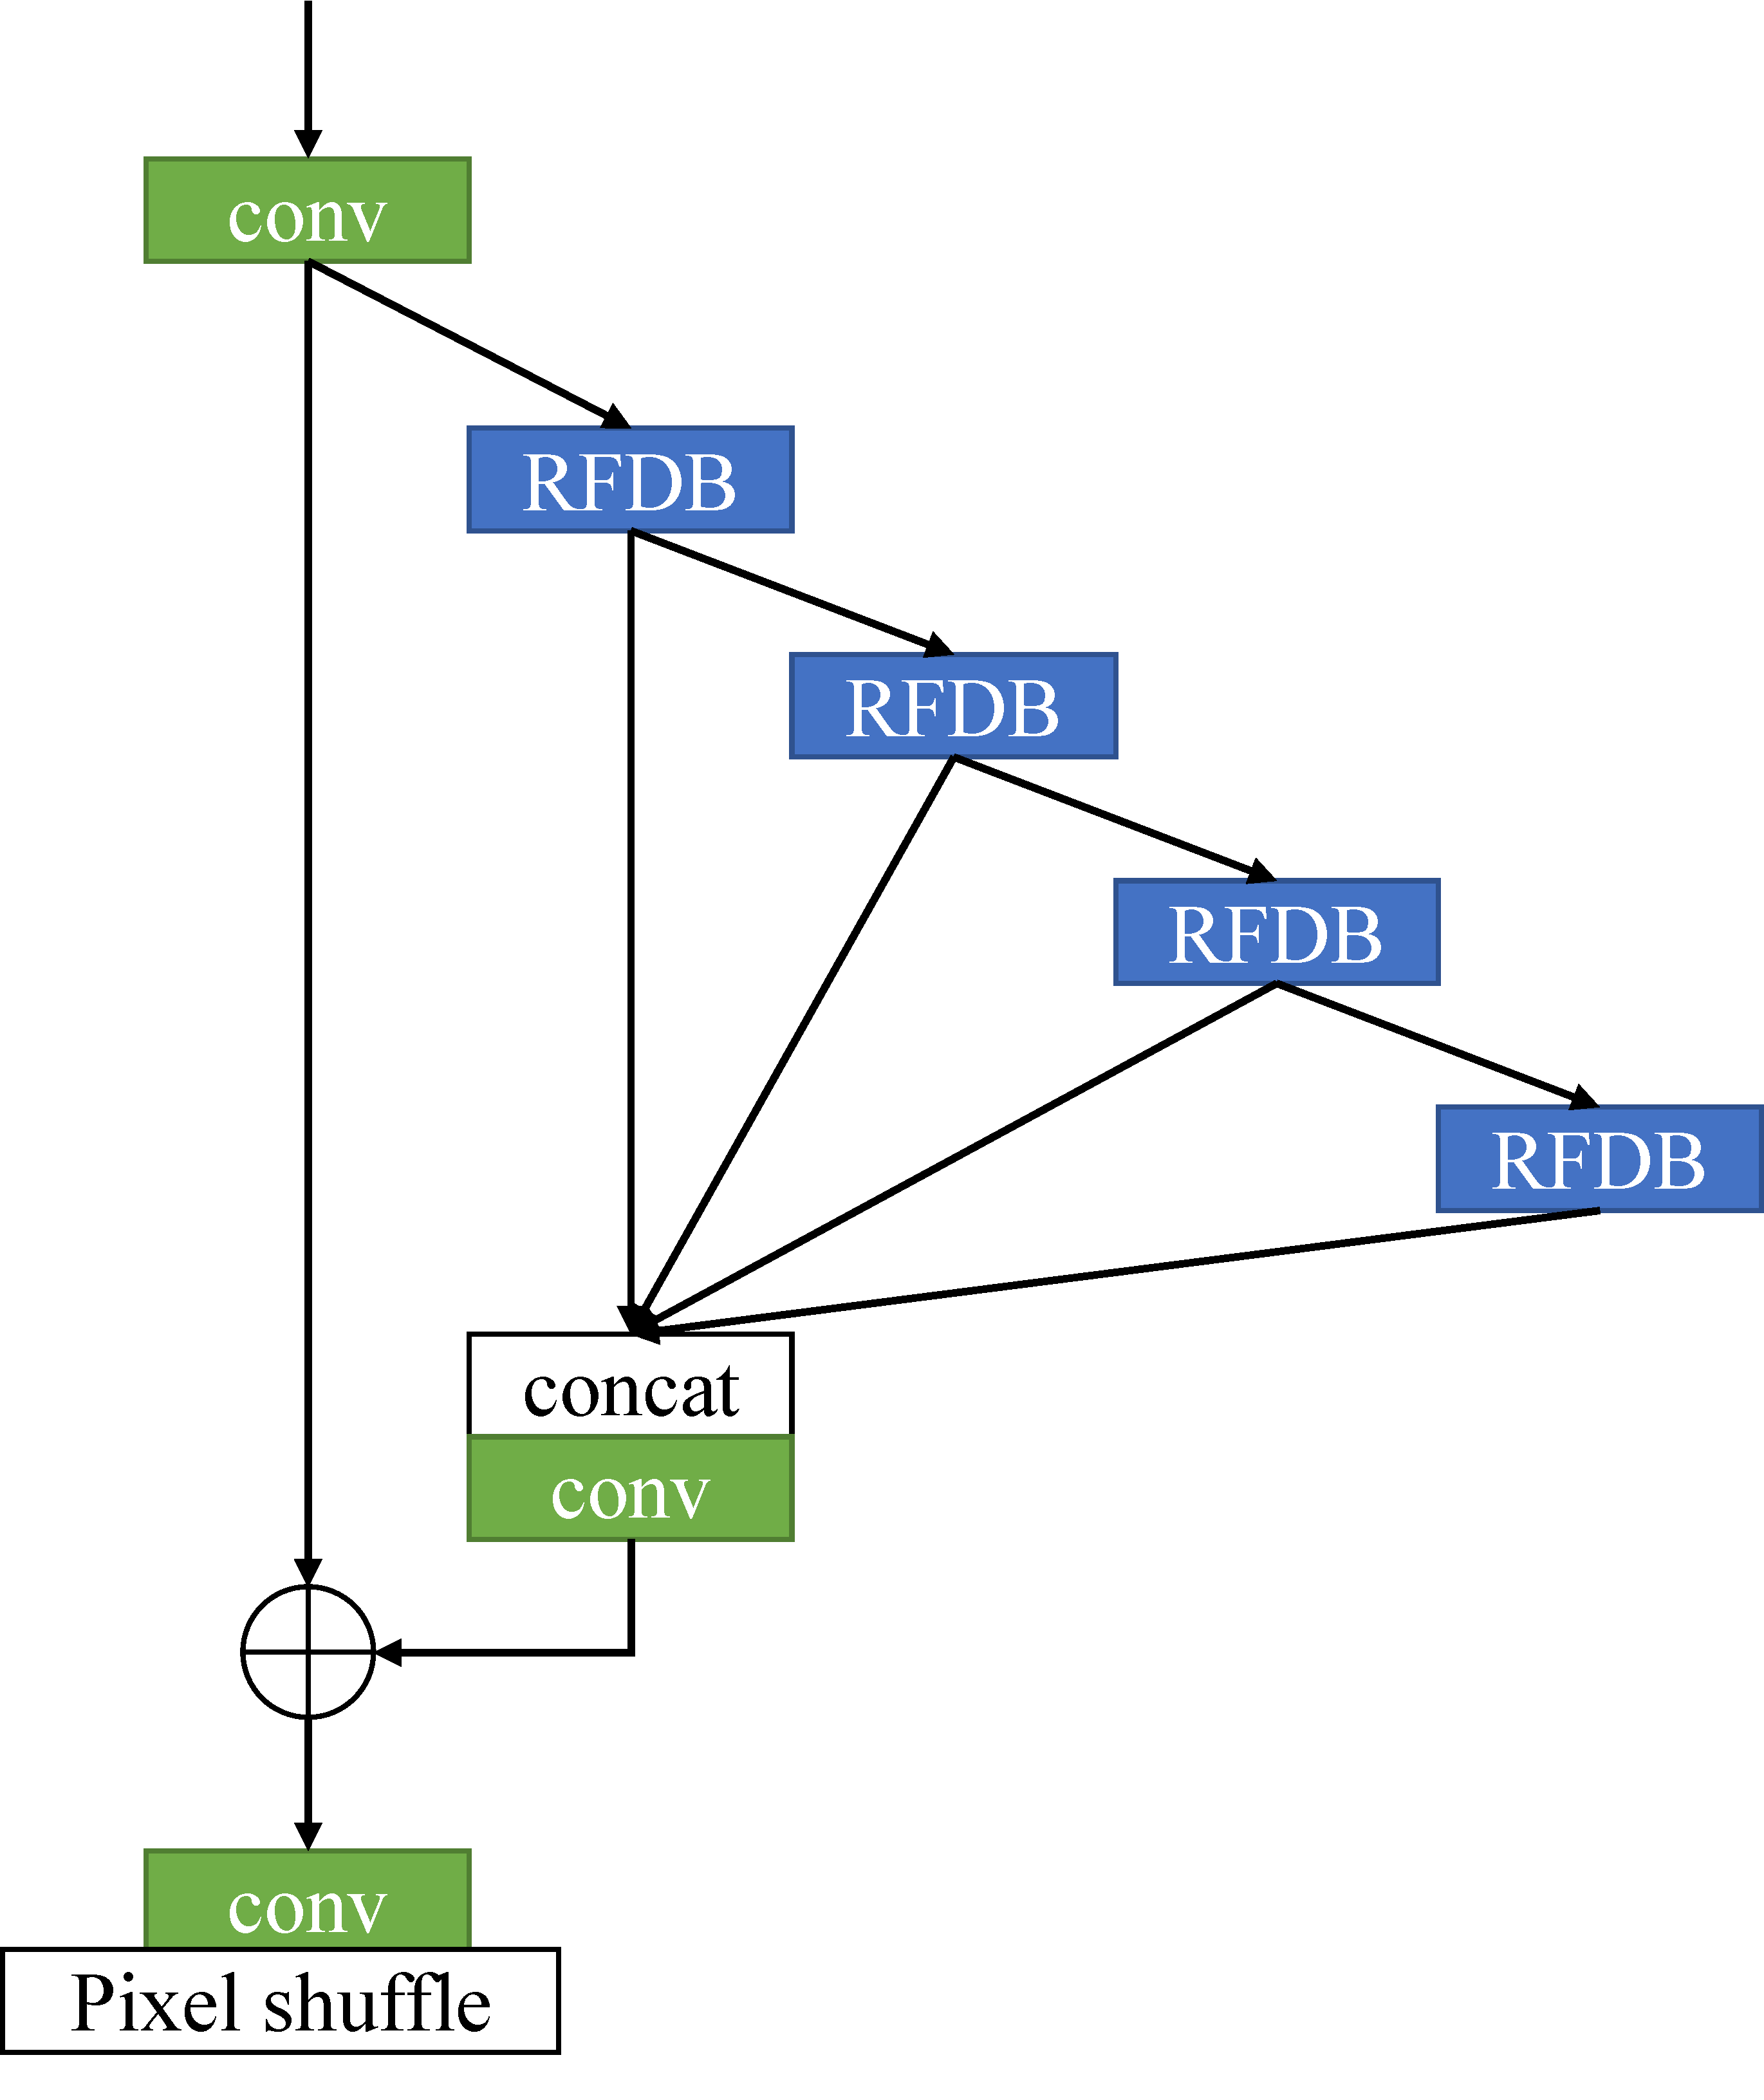
\includegraphics[width=\textwidth]{../RFDN.pdf}
        \caption{RFDN}
        \label{fig:RFDN}
    \end{subfigure}
    \begin{subfigure}[b]{0.2476\linewidth}
		\centering
        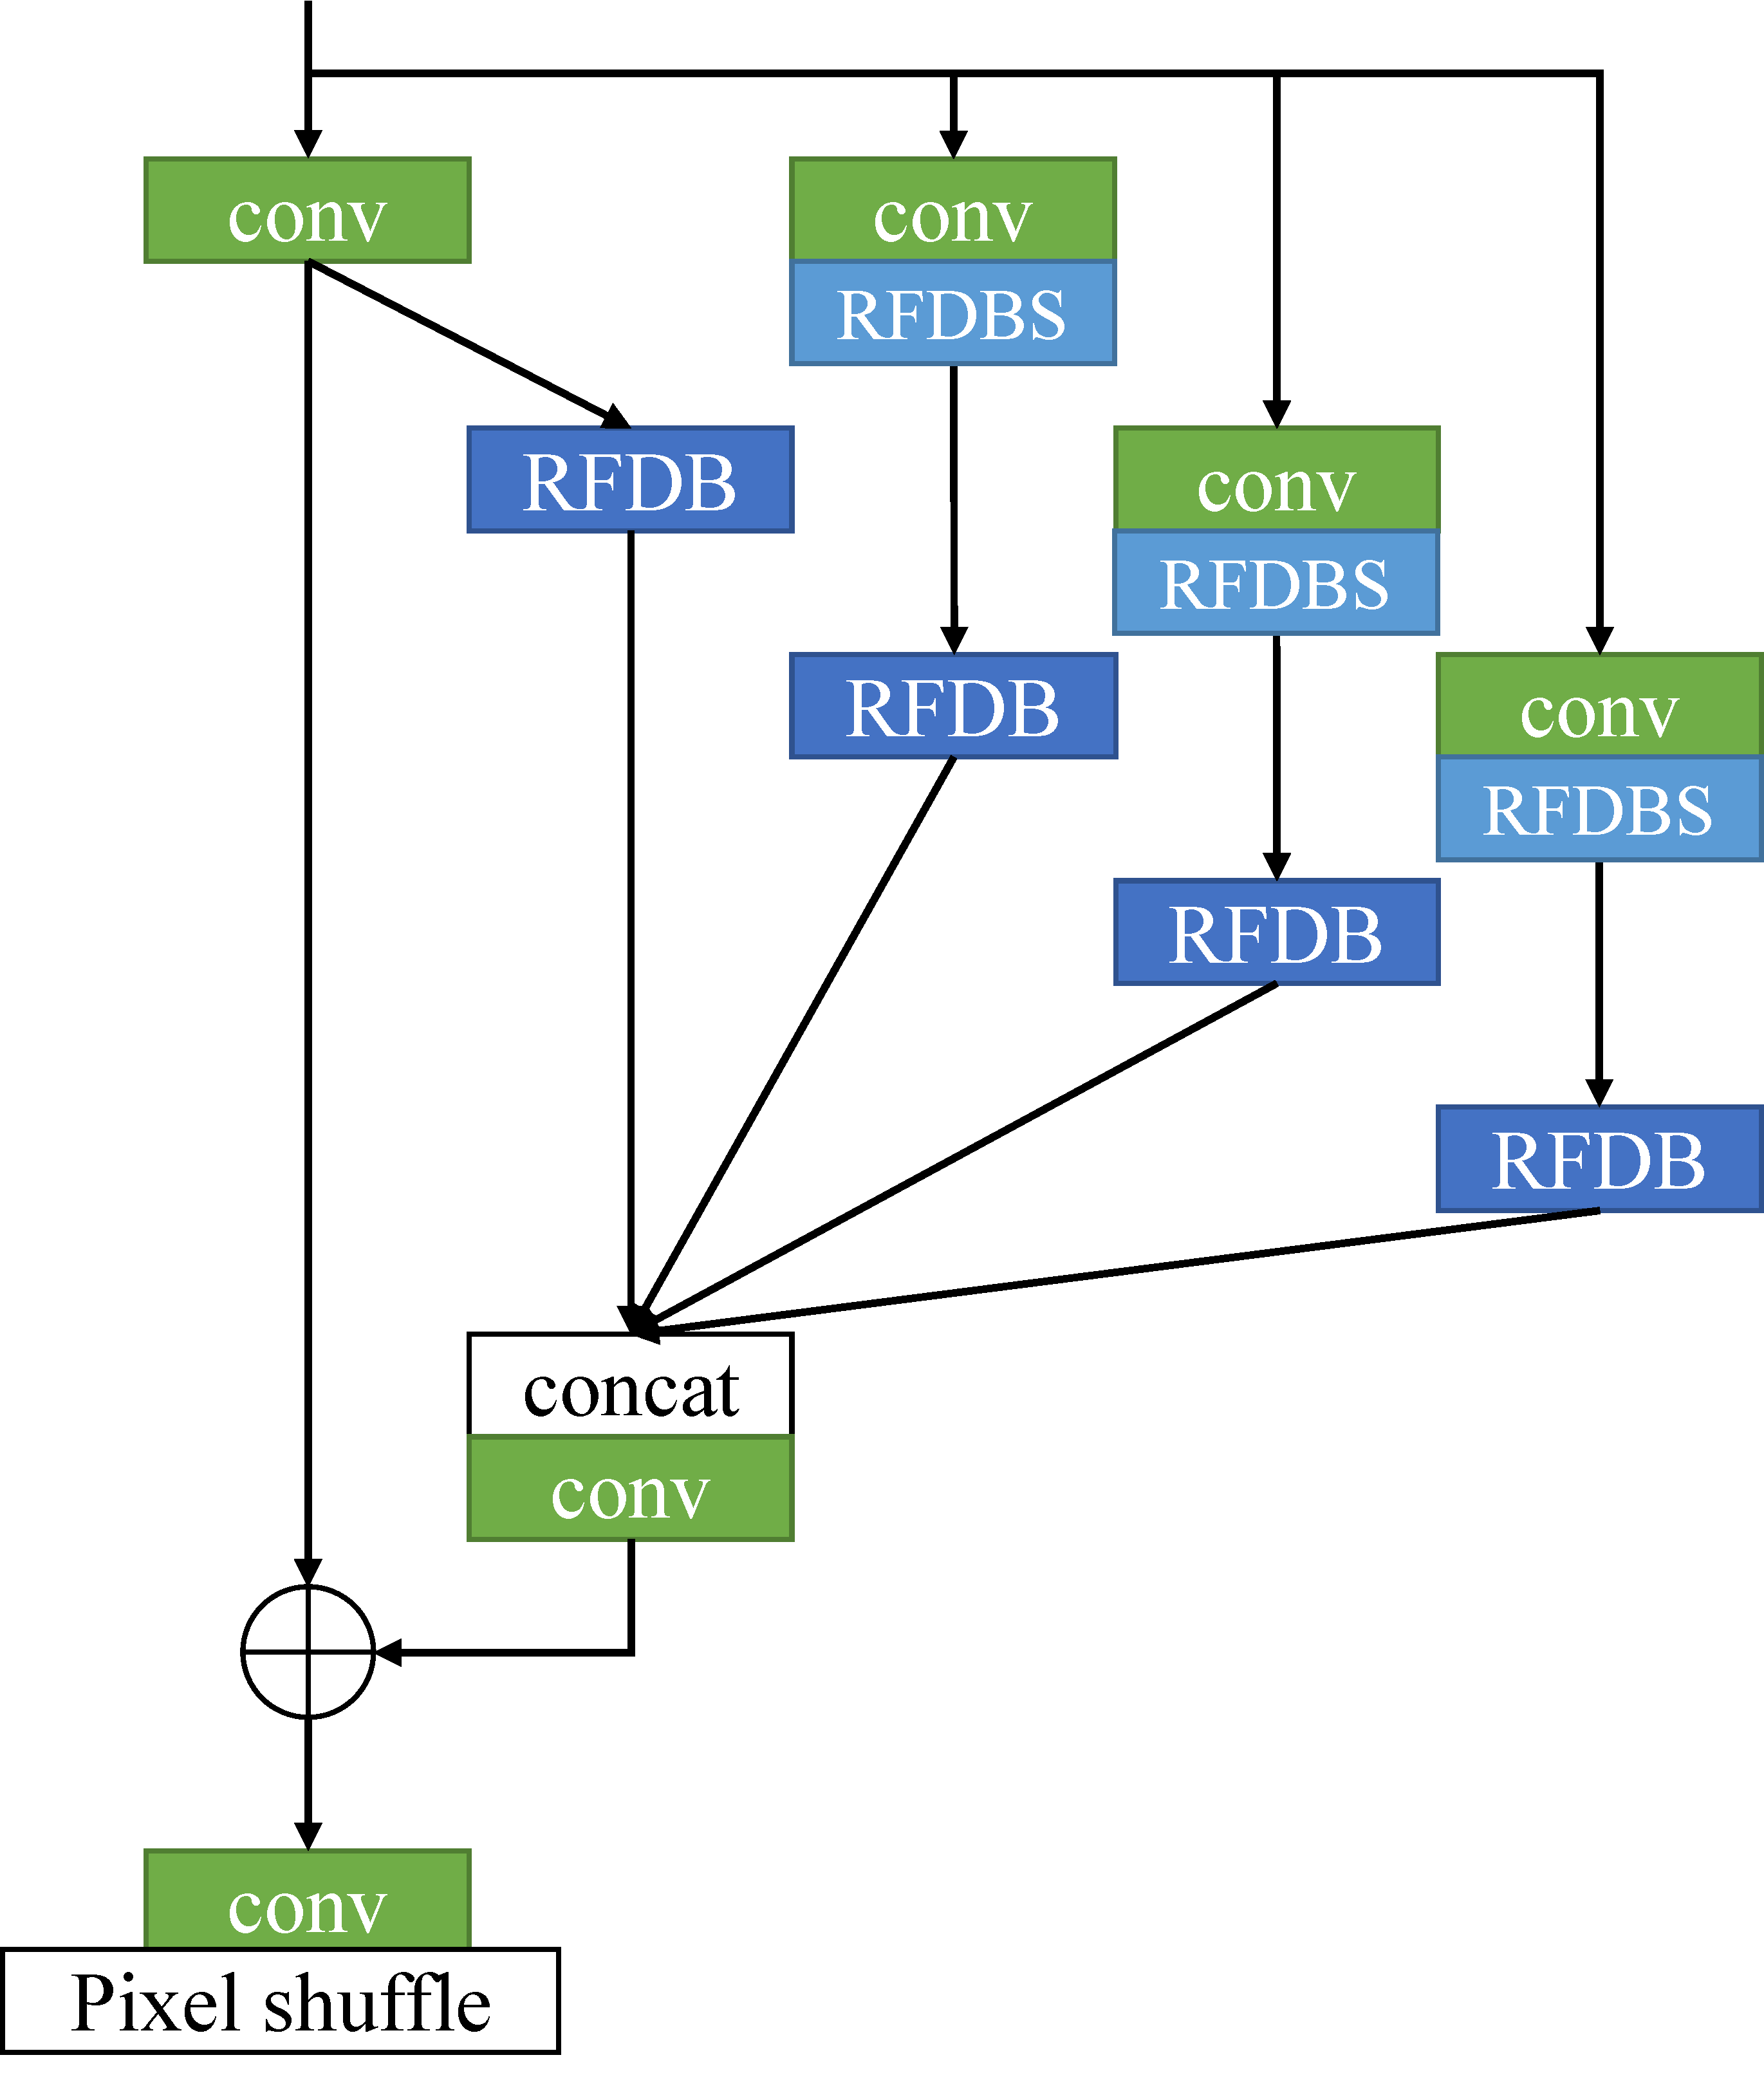
\includegraphics[width=\textwidth]{../Branching.pdf}
        \caption{Branching}
        \label{fig:Branching}
    \end{subfigure}
    \begin{subfigure}[b]{0.246\linewidth}
		\centering
        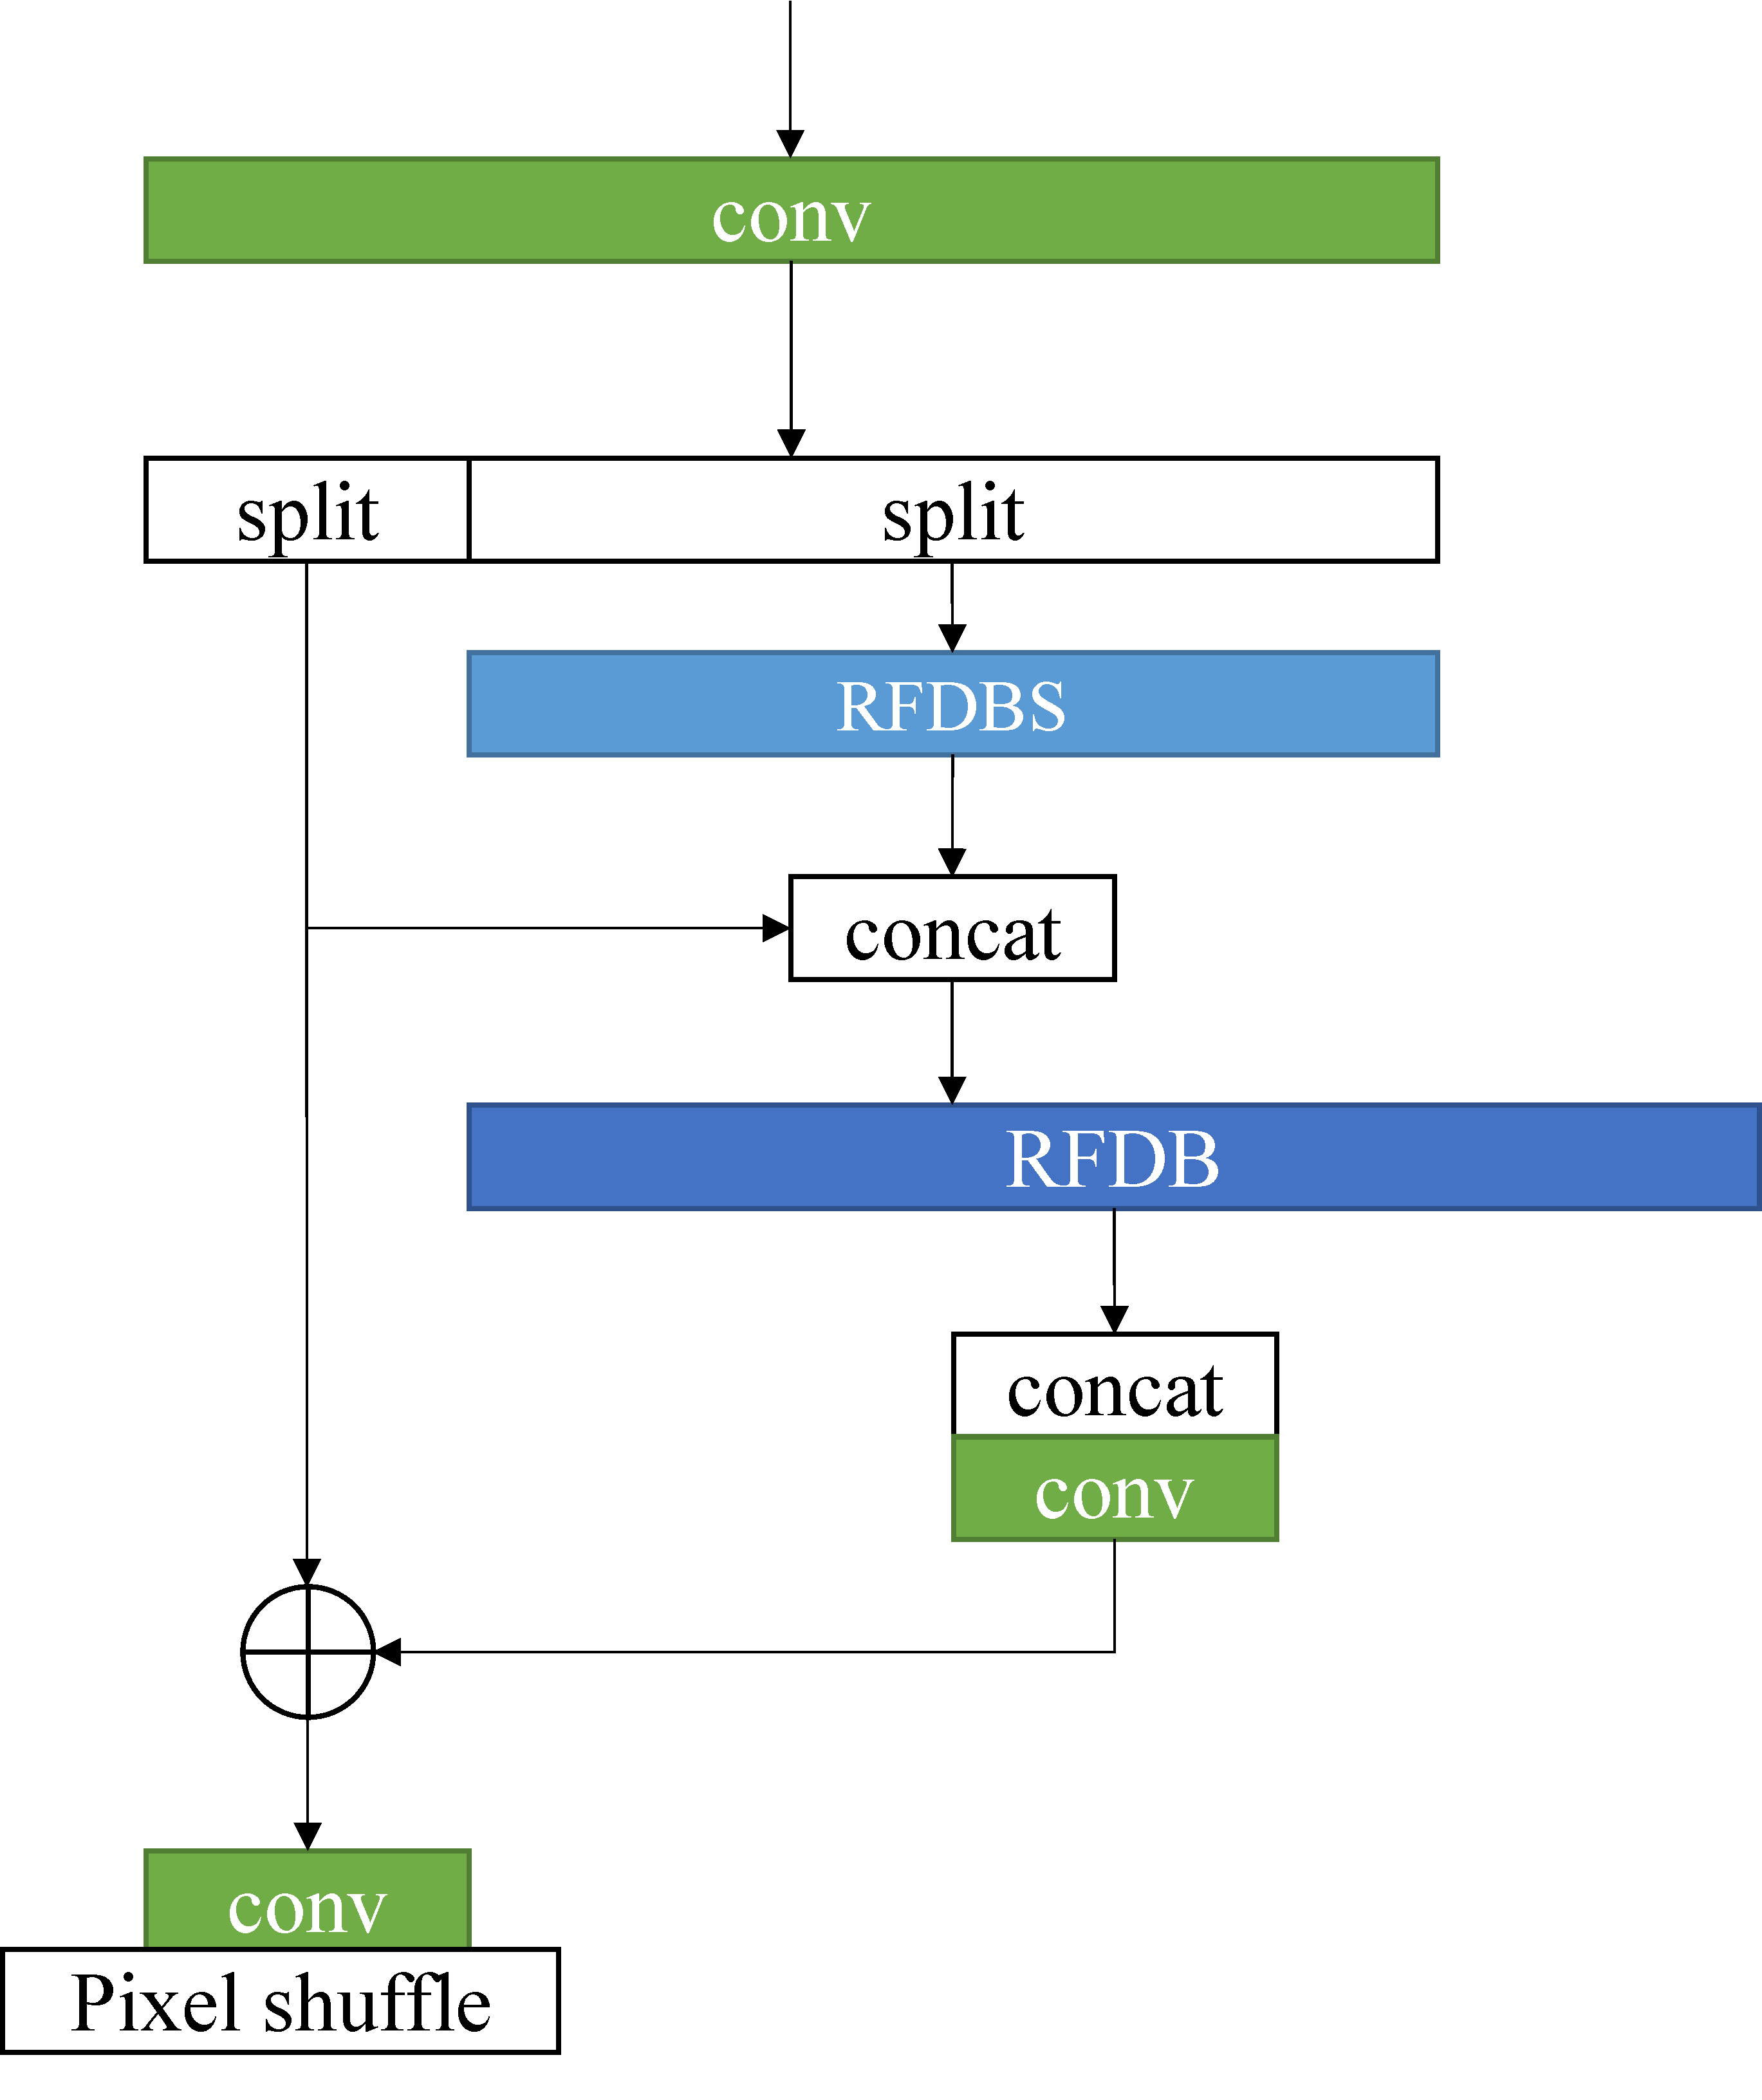
\includegraphics[width=\textwidth]{../Re-parametrization.pdf}
        \caption{Re-parametrization}
        \label{fig:Re-parametrization}
    \end{subfigure}
    \begin{subfigure}[b]{0.246\linewidth}
		\centering
        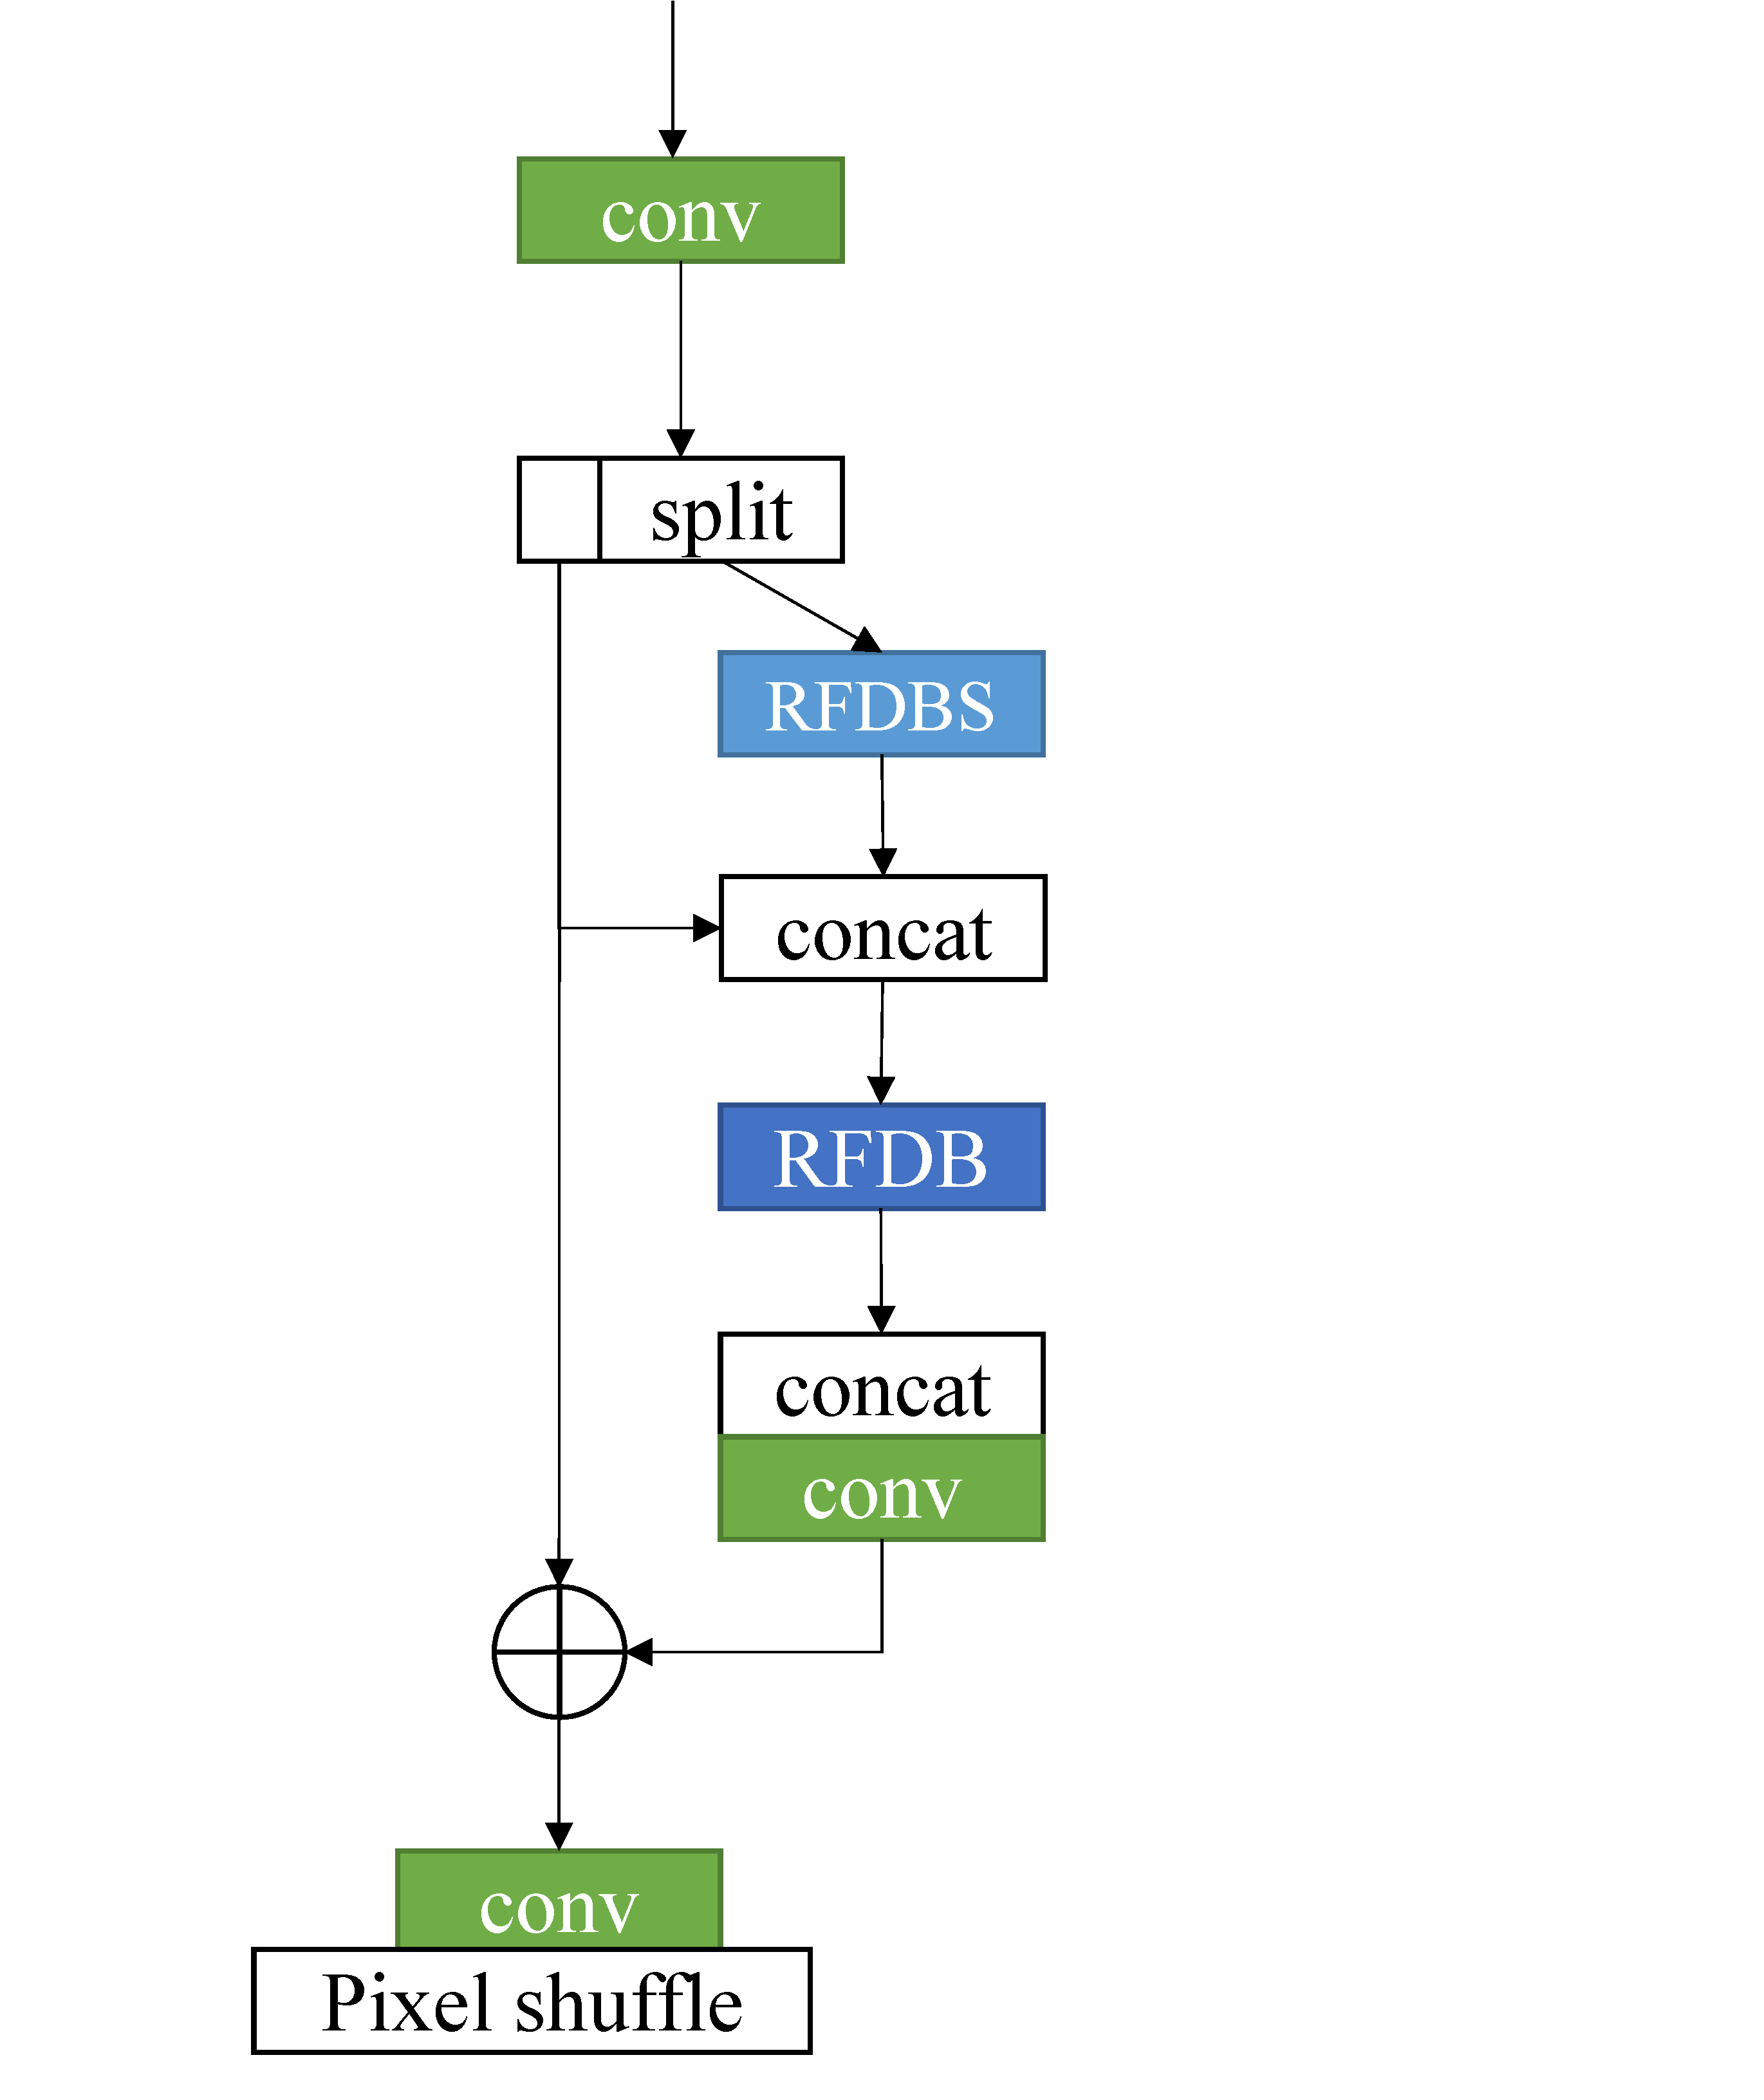
\includegraphics[width=\textwidth]{../Pruning.pdf}
        \caption{Pruning}
        \label{fig:Pruning}
    \end{subfigure}
    \caption{Transform a pre-trained RFDN into PRFDN}
    \label{fig:PRFDN}
\end{figure*}


\section{Technical details}
\begin{itemize}
    \item Language: Python
    \item Framework: Pytorch, Torch-Pruning\cite{fang2023depgraph}
    \item Optimizer: AdaM
    \item Learning rate\\Before re-parametrization: 1e-5 in general, if the loss cannot decrease after a lot of epochs, then descrease to 5e-6\\After re-parametrization: 1e-6
    \item GPU: RTX 3070 8G
    \item Datasets for training: LSDIR and DIV2K
\end{itemize}

\section{Other details}
\begin{itemize}
\item Planned submission of a solution(s) description paper at NTIRE 2023 workshop. YES
\item General comments and impressions of the NTIRE 2023 challenge. 

Positive impression: Scripts for running the models and measuring metrics are well organized.

Negative impression: Instructions are not clear (e.g. there are some posts in the forum saying that they cannot find the test set, but none of the organizers respond).

A small suggestion: Create a group in instant messaging apps (e.g. Discord or Telegram) for convenient communication.

\item What do you expect from a new challenge in image restoration, enhancement and manipulation?
Real-time video super-resolution; Efficient compressed video restoration.
\item Other comments: encountered difficulties, fairness of the challenge, proposed subcategories, proposed evaluation method(s), etc. N/A
\end{itemize}

%%%%%%%%% REFERENCES
{\small
\bibliographystyle{ieee_fullname}
\bibliography{egbib}
}

\end{document}
